%===================================================
%导论
\section  {INTRODUCTION}

%\section*{不编号的章节标题}
%\addcontentsline{toc}{INTRODUCTION}{不编号的章节标题}
%-------------------------------------------------
%问题重定义
\subsection{Restatement of the problems}
\par
\lettrine[lines=2]{T}{oday},information has many channels to spread and to be recieved. To explore the relationship between information's disseminating speed and its inherent value, make clear the revolution of methodology, purpose, and functionality of society's networks, we design some models to analysis the problems. They are designed based on a consideration of 5 periods: 1870s (Newspapers and Telegraph Age), 1920s (Radios Age), 1970s (Televisions Age), 1990s (Early Internet Age) and 2010s (Mobile Internet Age); 

\par Specifically, we face five subproblems:
\begin{itemize}
\item Develop one or more model(s) to explore the flow of information and filter;
\item Validate the models' reliability by using data from the past and the prediction capability of the model to predict the information communication situation for today and compare that with today's reality;
\item Use the model to predict the communication networks' relationships and capacities around the year 2050;

\item Use the theories and concepts of information influence on networks to model how public interest and opinion can be changed through information networks in today's connected world;

\item Determine how information value, people's initial opinion and bias, form of the message or its source, and the topology or strength of the information network in a region, country, or the world could be used to spread information and influence public opinion. 
\end{itemize}


\subsection{Backgrounds}
\par
From an historical perspective, whenever a new medium reaches critical mass it threatens to, and does, displace existing media to some degree. For instance, the upstart television industry took consumers and advertisers away from the radio industry back in the 1940s and 1950s.The revolution of special-interest niche magazines began back in the early 1970s; the magazine industry reacted to the loss of national advertising and eventual failure of mass circulation, general interest magazines due to the increasing use of television by both consumers and advertisers. The similar incident happened again when the Internet and the mobile Internet came into being.

\par These revolution seem to make it easier and sooner to gain news, but the inherent value of them seem to decrease because of the lower cost to make fake ones .What's worse , if someone has no idea of buying newspaper in the past ,people around him will discuss and tell him as a filter . But it doesn't work today .Software, websites and apps in mobile phones always remind you that something has happened no matter whether you would like to read.

\par Not every region enjoy the convenient communication network .In this context, the information explosion seems not so disgusting.
 %-------------------------------------------------
 \subsection{Our work}

 
 \par We consider that the problems are progressive , which contributes to solve the main problem. To analyze the relationship between speed/flow of information versus inherent value of information of 5 periods and solve all problems, we should firstly know the basic definitions and how dissemination work. Then, we should make clear its development over time relative to its scale, spreading speed and impact. Subsequently, we discuss how to changed people's mind through the Internet and how the dissemination of information. Finally, we make a brief conclusion of models, apply them to some "What if" problems and summarize the whole passage.
 
 \par In the part of modeling the dissemination , we firstly use the SW Model and BA Model. Then, we analysis the two models and combine them with some notions from Neural Networks into a modified model. After that, we discuss the filter and add them into the modified model. This is the basis for our further work.
 
 \par In the part of exploring the development, we make a prediction model inspired by the logistic model, the GM(1,n) Model and the BP model. These three basic models could describe our previous model in different perspectives, which are good reference to make a new model to describe the growth of information networks. Some data is used as validating the model, and some predictions are generated by the model.
 
 \par In the part of discussing the impact of information networks, we analysis the factors that change public interest and opinion, and model how to change it. Then, we discuss the information value, people's initial opinion and bias, form of the message or its source, and the topology or strength of the information network could be used to spread information and influence public opinion. We apply principal component analysis (PCA) to the first problem, the analytic hierarchy process (AHP) and a graphic model to the second problem. We discuss these problems within the scope of the world. Different analysis method reveals different facet of a problem, thus we no longer modified these methods.

 
 \par According the models made above, we tend to answer some "What if" problems, then state the models' strengths and weaknesses and make a conclusion of our whole work. 
 
 
%===================================================
%假设和参数

\subsection{Definitions}
\subsubsection*{What is "News"?}
News is packaged information about current events happening somewhere else; or, alternatively, news is that which the news industry sells. News moves through many different media, based on word of mouth, printing, postal systems, broadcasting, and electronic communication.

\subsubsection*{How to judge "Value"?}
\begin{itemize}
	\item Timeliness: a message should tell a recent story.
	\item Regionality: a story might happened in some region, and only affects the local people. The affected range shows a message's regionality.
	\item Significant: unimportant things is not worth mentioning.
	\item Abnormality: common things do not worth mentioning.

\end{itemize}
\par In general is, the greater the scope affected by the news event, the more people pay attention to the news event, the greater the value of it.

\subsubsection*{How to judge "Impact"?}
\par Impact is referred to the capability of letting the news be more known.In this essay, we consider it is equivalent to "Value".

%===================================================
%问题分析



\section{THE MODEL OF DISSEMINATION} 
\subsection{Assumptions}
\begin{itemize}
	\item Three roles take part in the dissemination of news:source, media and individual.
	\item Different types of roles' impact vary from one from another, while in a same type, different nodes' impact vary from one to another.
	\item The dissemination of information is with randomicity.
	\item The size of a node shows its impact.
	\item A line represents a two-way propagation. Each time, the direction of propagation depends on which node has greater influence.
\end{itemize}

\subsection{The initial models}
\subsubsection*{Parameters}
\begin{itemize}
	\item[-] $Node$ :The smallest unit of the dissemnation.
	\item[-] $Path$ :The smallest unit of the transmission of information.
	\item[-] $N$ :The number of nodes.
	\item[-] $L$ :The distance between two nodes.
	\item[-] $P$ :The randomness to attach to a new node.
	\item[-] $k$ :The total connections between nodes.
\end{itemize}

\subsubsection*{Model 1:The WS Model in Small-world Network}

A small-world network is a type of mathematical graph in which most nodes are not neighbors of one another, but most nodes can be reached from every other by a small number of hops or steps. $Watts$ and $Strogatz$ then proposed a novel graph model, currently named "the Watts and Strogatz (WS) model", with  a small average shortest path length, and a large clustering coefficient. Specifically, a small-world network is defined to be a network where the typical distance $L$ between two randomly chosen nodes (the number of steps required) grows proportionally to the logarithm of the number of nodes $N$ in the network.
\par In this model, we use different level of blue color to mark different roles in dissemination. The model is built from:
\begin{figure}[h]
	\small
	\centering
	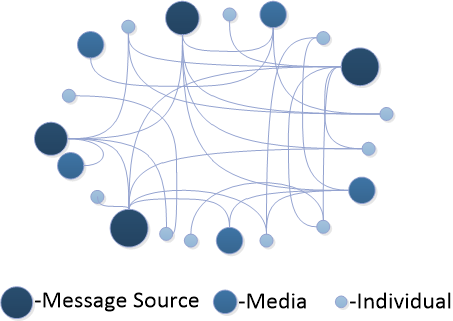
\includegraphics[width=9cm]{./picture/smallworld.png}
	\caption{The Small-world Model} \label{fig:Small-world Model}
\end{figure}
\begin{itemize}
\item a regular network which has $N$ points.
\item reconnect the nodes randomly. We have a coefficient $P$, which indicates the randomness as $(1)$:
\[
	P\in \left ( 0,1 \right ) \eqno(1)
\]
The distance between two nodes follow $(2)$:
\[
L\propto logN \eqno (2)
\]
\end{itemize}


\subsubsection*{Model 2:The BA Model in Scale-free Network}
 \begin{figure}[h]
 	\small
 	\centering
 	\includegraphics[width=12cm]{./picture/bamodel.png}
 	\caption{The BA Model} \label{fig:Scale-free network}
 \end{figure}
A scale-free network is a network whose degree distribution follows a power law, at least asymptotically. That is, the fraction $P(k)$ of nodes in the network having $k$ connections to other nodes goes for large values of $k$ as $(3)$
\[
P\left (k\right ) \sim k^{-\gamma } \eqno (3)
\]
where $\gamma$ is a parameter whose value is typically in the range as $(4)$ although occasionally it may lie outside these bounds.  
\[2\leq \gamma \leq 3\eqno(4)\]
\par The  $Barab\acute{a}si-Albert$ (BA) model is an algorithm for generating random scale-free networks using a preferential attachment mechanism. It is one of several proposed models that generates scale-free networks. Growth means that the number of nodes in the network increases over time. The model is built from:
\begin{itemize}
\item New nodes are added to the network one at a time. Each new node is connected to existing nodes $m< m_{0}$ with a probability that is proportional to the number of links that the existing nodes already have. 
\item Formally, the probability $P_{i}$ that the new node is connected to node where $i$ is 
\[P_{i}=\frac{k_{i}}{\Sigma _{j}k_{j}}\eqno (5)\]
$k_{i}$ is the degree of node $i$ and the sum is made over all pre-existing nodes Heavily linked nodes ("hubs") tend to quickly accumulate even more links, while nodes with only a few links are unlikely to be chosen as the destination for a new link. 
\item The new nodes have a "preference" to attach themselves to the already heavily linked nodes.
\end{itemize}
\par The degree distribution resulting from the BA model is scale free, in particular, it is a power law of the form. In this model,$\gamma$ is $3$.

\subsection{Analyse}
\par The WS model in Small-world Network and the BA model Scale-free Network partly reveal some features of a network of communication such as its topology.
\par The WS Model emphasizes the relationship of pairs of nodes and their reconnections. To show the randomness, the WS Model add its paths randomly to a previous one, and derive as NW Model. The degree of nodes are similar due to its building way. Unfortunately, its nodes will never increase by time and each added path doesn't have any preference. That is, we can consider all nodes in a same scale in this model actually.  
 
\par The BA Model pays attention on a "preferable" growth. The more degrees a node with, the more easily obtain a new path. If we take the degrees of a node to measure its impact, the more points it can affect, the easier to attach to a new node. However, in this model, the lager a node is, the more degrees it has. It seems not totally fit for the reality.
\par In the reality, nodes should link to another one not only based on its size and a randomness, but also many realistic factors.
\subsection{The advanced model}
\subsubsection*{Parameters}
\begin{itemize}
	\item[-] $Node$ :The smallest unit of the dissemnation.
	\item[-] $Path$ :The smallest unit of the transmission of information.
	\item[-] $N$ :The number of nodes.
	\item[-] $L$ :The distance between two nodes.
	\item[-] $P$ :The randomness to attach to a new node.

		\item[-] $F(t)$ :A function  reveals the time's affect
		\item[-] $k$ :The total connections between nodes.
	\item[-] $Direct Path$  :The unit which firstly reach the information source
	\item[-] $M/I Path$  :The process of information from a public media to an individual
	\item[-] $I/I Path$  :The process of information from an individual to another individual.
\end{itemize}
\subsubsection*{The modified model}
\begin{figure}[h]
	\small
	\centering
	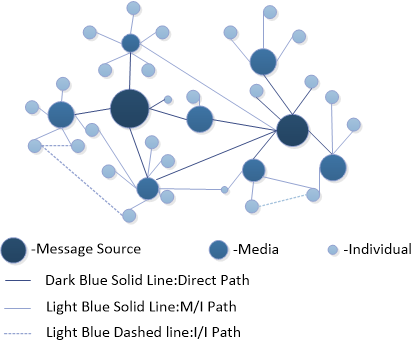
\includegraphics[width=12cm]{./picture/chuanbo.png}
	\caption{The Modified Model of the Dissemination Network} \label{fig:dissemination network}
\end{figure}
\par We combine the WS Model and the BA Model and some ideas such as parallel and the period of exciting and plain from Artificial Neural Network. The model can be described as follows:

\begin{itemize}
	\item Information can pass between individual and individual, between media and individual, between individual and source, and between media and source.
	
	\item Nodes are growing and the paths are growing depending on the speed of communication and the impact of a node over time.
		\begin{itemize}
			\item The speed of a flow depends on different tools.
			\item The scale of a node reveals its impact. If a node has more impact, it would be more easier to attached to another new node in a random.
			\item The information's passing will die out over time, as:
			\[F_{\left (t \right )}\propto t \eqno (6)\]
		\end{itemize}
	\item The growing is in parallel of a randomness $P_{i}$,as
	\[P_{i}=\frac{I_{i}}{\Sigma _{j}I_{j}}\eqno (7)\]
	As a result,the growth of the model is:
	\[V_{G}=V_{c}\times P_{i}\times F_{\left (t \right )}\times Value\eqno (8)\]
	That is:
	\[V_{G}=V_{c}\times \frac{I_{i}}{\Sigma _{j}I_{j}}\times F_{\left (t \right )}\times Value\eqno (9)\]
\end{itemize}

\par 
\subsubsection*{The shilter}
\par 
According to the definitions, we know that not all information qualifies news. News is packaged information about current events happening somewhere else; or, alternatively, news is that which the news industry sells. Obviously, the news industry is a filter of information.
\subsubsection*{The modified model with filters}\begin{figure}[h]
	\small
	\centering
	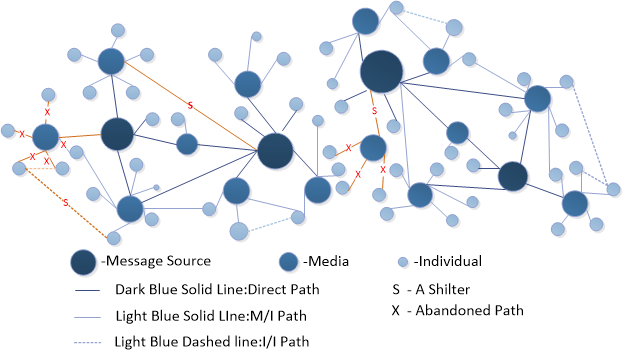
\includegraphics[width=15cm]{./picture/final1.png}
	\caption{dissemination network adding filters} \label{fig:dissemination network adding shilters}
\end{figure}
\par To determine filters' role in news' broadcasting, the model of a modified one has been expanded. If one node take part as a filter, then other nodes connect with it couldn't get the news unless it connects to another active node.




\section{THE DEVELOPMENT OF INFORMATION NETWORKS}

\subsection{Assumptions}
\begin{itemize}
	\item The prediction model in this part is based on the modified dissemination model with filters. (The flow of news)
	\item To simplify the problem, we only consider the revolution's interval, the spreading speed and the value.
	\item We consider the spreading speed as a one-round spread cycle and a re-spread speed. 
	\item We consider the nodes' impact on how much time people spend on receiving news every week.
	\item The filter is ignored.
	\item In this part, fading-out of a flow of information is ignored.
\end{itemize}
\subsection{The initial models}
\subsubsection*{Parameters}
\begin{itemize}
	\item[-] $N$ :The number of factors.
	\item[-] $m$ :The number of periods.
	\item[-] $n$ :The length of time.
\end{itemize}
\subsubsection*{Model 1: A model derived from logistic function}
\par
Logistic function or curve is a common S-shaped function, it is Pierre Francois Weilvle in 1844 or 1845 in the study of the relationship between population growths when it's named. Generalized Logistic curve can imitate some cases, population growth of the S-shaped curve. First phase is substantially exponentially; then started to become saturated with the increase slowed; and finally, increased stopping reach maturity. Biological growth process experience, development to maturity in three stages.
\par This model mainly contributes to measure a single feature.
\par A raw fuction is:
\[
y=\frac{1}{K+ab^{t} }  \eqno (10)
\]
where
\[
K>0,a>0,0<b\neq 1
\]
Then,
\[y_{t}^{'}=K+ab^{t}\eqno (11)\]
We thus obtained their arguments from:
\[\left\{\begin{matrix}
&b=&\left ( \frac{S_{3}-S_{2}}{S_{2}-S_{1}} \right )^{\frac{1}{m}}   \\ 
&a=&(S_{2}-S_{1})\frac{b-1}{b\left ( b^{m}-1 \right )^{2}} \\
&  K=&\frac{1}{m}
\end{matrix}\right.\eqno (12)
\]
where\[S_{1}=\sum_{t=1}^{m}y^{'}_{t},S_{2}=\sum_{t=m+1}^{2m}y^{'}_{t},
S_{3}=\sum_{t=2m+1}^{3m}y^{'}_{t}\eqno(13)\]
	\par In this model, we consider five periods from 1920s to 2010s. $n$ is $90$ while $m$ is $5$.


\subsubsection*{Model 2: Grey Prediction Model}
\par Grey prediction is a system containing uncertainties method to predict. Grey model was developed from the grey system theory introduced by Deng in the early 1980s. It can be used to predict behaviors of systems in the future value with high accuracy without knowing their mathematical models and used in the uncertain coefficients system with small nonnegative data. Grey model has been successfully applied to various systems. $GM(m,n)$ denotes a grey model which indicates that  variables are employed in the model and that it is an $m$-order differential equation. $GM(1,1)$ is a first-order one-variable grey differential equation, and it is the most widely used grey model in time series prediction. $GM(1,n)$ model is a grey multivariable model used for estimating the relationship between the system behavior and  relative factors and has been used for various applications, we adapt this model as a basic model.
\begin{itemize}
	\item From the assumptions, the $N$ behavior factors specifically can be:the scale,the growing speed and the inherent value.The original sequence is($N$ equals 4):
	\[
	x_{i}^{\left ( 0 \right )}=  \left ( x_{i}^{\left ( 0 \right )}  \left ( 1 \right ) ,  
	x_{i}^{\left ( 0 \right )}  \left ( 2 \right )
	x_{i}^{\left ( 0 \right )}  \left ( 3 \right )
	x_{i}^{\left ( 0 \right )}  \left ( 4 \right )                   
	\right )\eqno (14)
	\]
	where $i=1,2,3,4$
	The AGO transformation is defined as: 
	\[x_{i}^{\left ( 1 \right )}=  \left ( x_{i}^{\left ( 1 \right )}  \left ( 1 \right ) ,  
	x_{i}^{\left ( 1 \right )}  \left ( 2 \right )
	x_{i}^{\left ( 1 \right )}  \left ( 3 \right )
	x_{i}^{\left ( 1 \right )}  \left ( 4 \right )                   
	\right )\eqno(15)\]
	
	That is:
	\[x_{i}^{\left ( 1 \right )}  =
	\left ( x_{i}^{\left ( 1 \right )}  \left ( 1 \right ) ,x_{i}^{\left ( 1 \right )}  \left ( 1 \right )+  
	x_{i}^{\left ( 0 \right )}  \left ( 2 \right ),x_{i}^{\left ( 0 \right )}  \left ( 2 \right )
	+
	x_{i}^{\left ( 1 \right )}  \left ( 3 \right ),x_{i}^{\left ( 1 \right )}  \left ( 3 \right )
	+
	x_{i}^{\left ( 0 \right )}  \left ( 4 \right ),x_{i}^{\left ( 0 \right )}  \left ( 4 \right )                   
	\right )\eqno(16)
	\]
	where $i=1,2,3,4$
	while
	\[x_{i}^{\left (1  \right )}\left ( k \right )=\sum_{j=1}^{k}x_{i}^{\left (0  \right )}\left ( j \right )    (k=2,3,4)\eqno(17)
	\]
	\item Then,we make $x_{i}^{\left (1  \right )}$ as:
	\[
	z_{1}^{\left (1  \right )}=0.5x_{1}^{\left (1  \right )}\left ( k \right )+0.5x_{1}^{\left (1  \right )}\left ( k-1 \right )(k=2,3,4)
\eqno(18)	\]
	\item Thus,we get $GM(1,n)$'s regression equation:
	\[x_{1}^{\left (0  \right )}\left ( k \right )+az_{1}^{\left (1  \right )}\left ( k \right )
	=\sum_{i=2}^{4}b_{i}x_{i}^{1}\left ( k \right )\eqno(19)\]
	
	$x_{1}^{\left (0  \right )}\left ( k \right )$ is the grey derivative,
	$z_{1}^{\left (1  \right )}\left ( k \right )$ is the background value,
	$a,b_{i}$ is a parameter.
	\item If we consider $k=1,2,3,……N$ as continuous variable $t$, the sequence $x_{i} ^{k}(k)$ can be considered as a function of $t$. Thus,we can get the white differential equation as:
	\[
	\frac{\mathrm{d}x_{1}^{\left ( 1 \right )} }{\mathrm{d}t}+ax_{1}^{\left (1  \right )}\left ( t \right )=\sum_{i=2}^{N}b_{i}x_{i}^{\left (1  \right )}\left ( t \right )
\eqno(20)	\] 
\end{itemize}
\subsubsection*{Model 3: The BP Model}
\par In machine learning and cognitive science, artificial neural networks (ANNs) are a family of models inspired by biological neural networks (the central nervous systems of animals, in particular the brain) and are used to estimate or approximate functions that can depend on a large number of inputs and are generally unknown. Artificial neural networks are generally presented as systems of interconnected "neurons" which exchange messages between each other. The connections have numeric weights that can be tuned based on experience, making neural nets adaptive to inputs and capable of learning.
\begin{figure}[h]
	\small
	\centering
	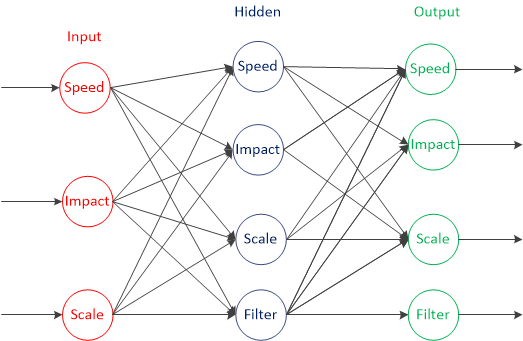
\includegraphics[width=12cm]{./picture/BPm.png}
	\caption{A initial BP Model}
	 \label{fig:A initial BP Model}
\end{figure}
In this model, some parameters can be defined as:
\[input=\sum_{i=1}^{3}input(i)\eqno(21)\]
\[hidden:n=\sqrt{\sum_{i=1}^{3}input(i)+4}\eqno(22)\]
where $i$ is shenjingyuanshuliang.
\[output(j)=\sum_{j=1}^{4}func\left ( n \right )\eqno(23)\]
where $func(x)$ is a function calculating the influence of $n$.
\subsection{Analyse}
\par Three basic models show different aspects of the dissemination. All of them can predict the trend of a flow of information with a small amount of data.

\par The model derived from logistic function mainly focuses on the growing of a system. The logistic function is a type of time series function model. In the first phase of it grows slowly, the development period is suddenly accelerated, and to maturity and tend to slow down, to form a S-shaped curve. We consider that it is a characteristic of network development. However,the parameters within the function is hard to determine. Besides, it's not a multivariable function.

\par The second model, we adapt a GM(1,n) model(one of grey prediction models).These factors affecting the growth have a certain degree of relevance. The model combines different factors to consider the development of dissemination and gives a result using small amount of data. What's more, we don't need to determine some parameters because the functions are determined, which reduces the subjectivity. The weakness is, its next result based on the previous one and ignore some random incidents which can totally change the growth.
\par The third model, the BP Model in artificial neural network. Artificial neural networks are generally presented as systems of interconnected "neurons" which exchange messages between each other. The connections have numeric weights that can be tuned based on experience, making neural nets adaptive to inputs and capable of learning. That is the reason we consider this model. The development of dissemination may has the feature of uncertain. A BP Model can predict its backwards development based on not a certain function, and output the result of different factors' development, which helps to measure the whole system. However, it's hard to determine a three input, four output model.

\subsection{The modified model}
\par We want to know each factor's development as well as the whole system's development. In order to outline their relationships, we modified a model which combined three models. We find that in a BP algorithm, a logistic function could be a motivation function. Consider the poor amount of data, we add the grey model to. Specifically, we put some data into a $GM(1,n)$ function to see a whole growth, then fixed the rounds of studying in the BP function.
\subsection{The Results}
\subsubsection*{Parameters}
\begin{itemize}
	\item $RI$:The interval between a revolution and a formal one.
	\item $OS$ : The interval from an incident occur to people can access to it.
	\item $RS$ :The interval from an incident being spread to another spreading.
	\item $RT$ :The time people spending on receiving news per week.
\end{itemize}
\subsubsection*{Validating and Prediction}
	\par We access some data from the Internet and make the average value as shown below:
\begin{table}[tbp]
	 \centering% 表居中
	\begin{tabular}{lccccc}  % {lccc} 表示各列元素对齐方式,left-l,right-r,center-c
		\hline
		Items & 1870s & 1920s & 1970s & 1990s & 2010s\\ \hline  % \hline 在此行下面画一横线
		RI (years) & 80 & 70  & 50  & 20 & 20 \\         % \\ 表示重新开始一行
		OS (hours)& 72 & 5 & 2 & 0.5 & 0.17\\        % & 表示列的分隔线
		RS (hours) & 158 & 48 & 24 & 3 & 0.5\\ 
		RT (hours) & 42 & 65 & 112 & 158 & 187  \\
		\hline
	\end{tabular}
	\caption{Data obtained through the Internet}\label{tab:1}
\end{table} 
\par Then ,we put them into our modified model, and get the result as:
\begin{figure}[h]
	\small
	\centering
	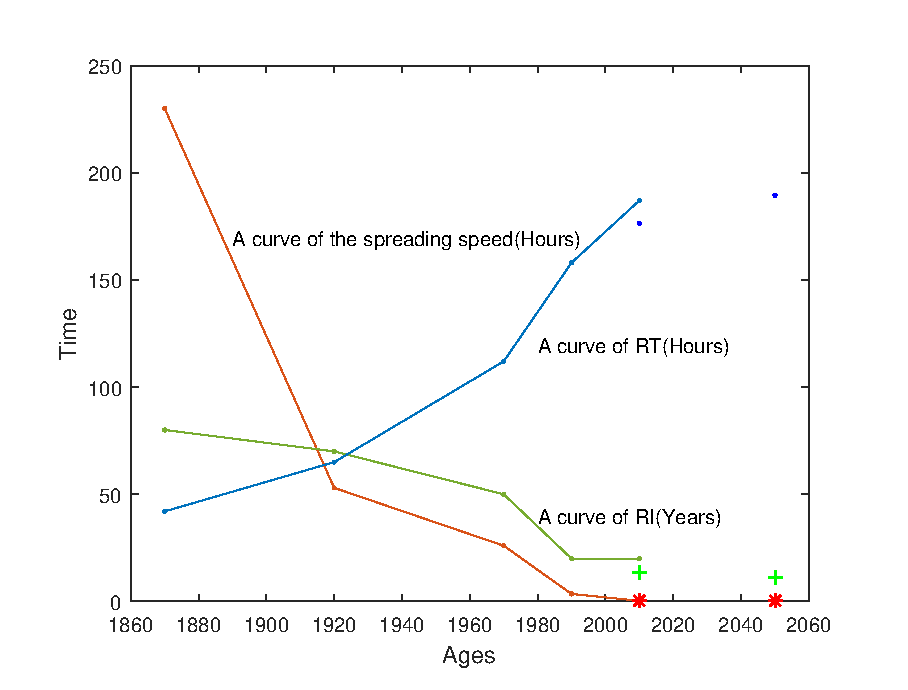
\includegraphics[width=15cm]{./picture/wtf.eps}
	\caption{The results}
	\label{fig:The results}
\end{figure}

\par Where the solid line the real data and the singles points are generated by the modified model.

\begin{table}[h-ere]
	\centering% 表居中
	\begin{tabular}{lccccc}  % {lccc} 表示各列元素对齐方式,left-l,right-r,center-c
		\hline
		Items & MSE & SSE   & RMSE\\ \hline  % \hline 在此行下面画一横线
		RI   & 40.4496  & 40.4496  & 6.3600 \\         % \\ 表示重新开始一行
		SS (hours)& 0.0121  & 0.0121 & 0.1100 \\        % & 表示列的分隔线
		RT (hours) & 111.7249 & 111.7249 & 10.5700   \\
		\hline
	\end{tabular}
	\caption{Data through the Internet}\label{tab:1}
\end{table} 
\par To confirm its capability of predicting, we use the $MSE,SSE,RMSE$ to measure the prediction model. The measure of the prediction error is shown in $Table 2$. As a matter of fact it doesn't seem to work,it tells nothing. We consider it's a result of the poor scale of data.
\subsection*{Extends}
\par Refer to the impact a dissemination network brings, we should consider in different periods, different devices show them in different ways. We find some data which reveals the impact of different periods of different devices as below:


\begin{figure}[h]
	\small
	\centering
	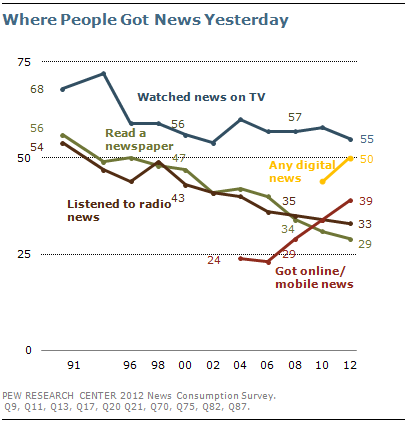
\includegraphics[width=10cm]{./picture/lala.png}
	\caption{Where to get news?}
	\label{fig:Where to get news?}
\end{figure}
\par Obviously, a new tool always attracts people's attention and people tend to get news in new ways.
\begin{figure}[h]
	\small
	\centering
	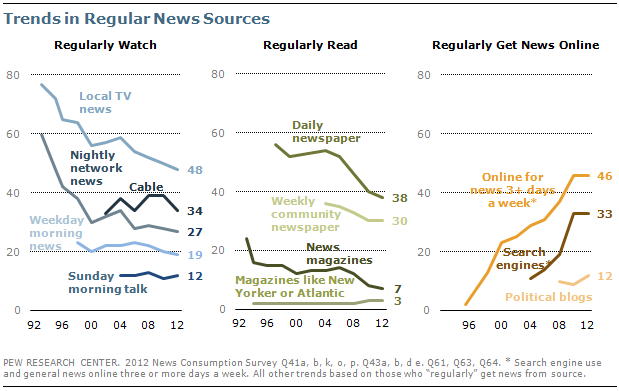
\includegraphics[width=11cm]{./picture/lala2.png}
	\caption{Trends}
	\label{fig:Trends}
\end{figure}



\section{THE INFLUENCE OF INFORMATION NETWORKS}
\subsection{An AHP MODEL to explore what makes a change}
\subsubsection *{The model}
\par The analytic hierarchy process (AHP) is a structured technique for organizing and analyzing complex decisions, based on mathematics and psychology. It was developed by Thomas L. Saaty in the 1970s and has been extensively studied and refined since then.
\par It has particular application in group decision making, and is used around the world in a wide variety of decision situations, in fields such as government, business, industry, healthcare, shipbuilding[2] and education.
\par Rather than prescribing a "correct" decision, the AHP helps decision makers find one that best suits their goal and their understanding of the problem. It provides a comprehensive and rational framework for structuring a decision problem, for representing and quantifying its elements, for relating those elements to overall goals, and for evaluating alternative solutions.
\par Step 1, a hierarchical structure model is established as:
\begin{figure}[h]
	\small
	\centering
	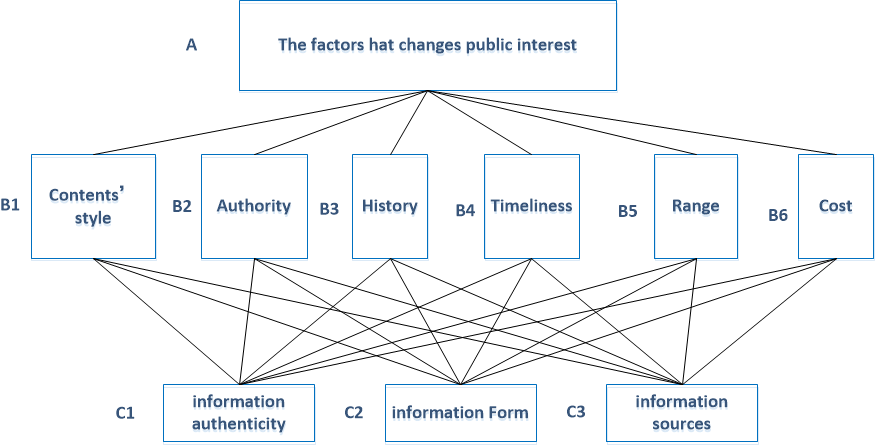
\includegraphics[width=15cm]{./picture/cengci.png}
	\caption{The AHP Model}
	\label{fig:The AHP Model}
\end{figure}

\par Step 2,the establishment of judgment matrix:
Establish the judgment matrix of the criterion layer according to the target and the criterion of the data list,as :

\begin{table}[h-ere]
	\centering% 表居中
	\begin{tabular}{lcccccc}  % {lcccccc} 表示各列元素对齐方式,left-l,right-r,center-c
		\hline
		A & B1 & B2   & B3 & B4 & B5 & B6\\ \hline  % \hline 在此行下面画一横线
		B1   & 1    & 1    & 1    & 4   & 1 & 1/2  \\      
		B2   & 1    & 1    & 2    & 4   & 4 & 1/2  \\   
		B3   & 1    & 1/2  & 1    & 5   & 3 & 1/2  \\   
		B4   & 1/4  & 1/4  & 1/5  & 1   & 1/3 & 1/3  \\   
		B5   & 1    & 1    & 1/3    & 3 & 1 & 1  \\   
		B6   & 2    & 2    & 2    & 3   & 3 & 1  \\       
		\hline
	\end{tabular}
	\caption{The judgment matrix of the criterion layer}\label{tab:3}
\end{table} 
	\par Step 3, the establishment of judgment matrix:
	Establish measure layer judgment matrix.
	
	
	% Table generated by Excel2LaTeX from sheet 'Sheet1'
	\begin{table}[htbp]
		\centering
		\begin{tabular}{rrrccccrccrc}
			\toprule
			B1    & C1    & C2    & C3    & B2    & C1    & C2    & \multicolumn{1}{c}{C3} & B3    & C1    & \multicolumn{1}{c}{C2} & C3 \\
			\midrule
			C1    & 1     &  1/4  &  1/2  & C1    & 1     &  1/4  & \multicolumn{1}{c}{ 1/5} & C1    & 1     & \multicolumn{1}{c}{3} &  1/3 \\
			C2    & 4     & 1     & 3     & C2    & 4     & 1     & \multicolumn{1}{c}{ 1/2} & C2    &  1/3  & \multicolumn{1}{c}{1} &  1/7 \\
			C3    & 2     &  1/3  & 1     & C3    & 5     & 2     & \multicolumn
			{1}{c}{1} & C3    & 3     & \multicolumn{1}{c}{1} & 1 \\ \hline \\ \hline
			B4    & C1    & C2    & C3    & B5    & C1    & C2    & \multicolumn{1}{c}{C3} & B6    & C1    & \multicolumn{1}{c}{C2} & C3 \\ \hline
			C1    & 1     &  1/3  & 5     & C1    & 1     & 1     & \multicolumn{1}{c}{7} & C1    & 1     & \multicolumn{1}{c}{7} & 9 \\
			C2    & 3     & 1     & 7     & C2    & 1     & 1     & \multicolumn{1}{c}{7} & C2    &  1/7  & \multicolumn{1}{c}{1} & 1 \\
			C3    &  1/5  &  1/7  & 1     & C3    &  1/7  &  1/7  & 1     & C3    &  1/9  & 1     & 1 \\
			\bottomrule
		\end{tabular}%
		\caption{The judgment matrix of the criterion layer}\label{tab:4}
	\end{table}%
	\par Then,we have the final result:
	% Table generated by Excel2LaTeX from sheet 'Sheet1'
	\begin{figure}[h]
		\small
		\centering
		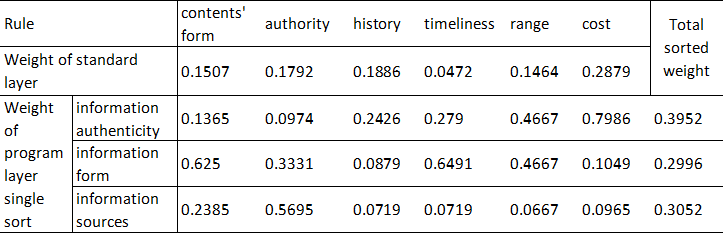
\includegraphics[width=15cm]{./picture/mmm.png}
		\caption{The AHP Model}
		\label{fig:The AHP Model}
	\end{figure}

\par In order to be more intuitive,we can seek the answer from the figure.
\subsection{A PCA Model to determine how to change}
\par Principal component analysis (PCA) is a statistical procedure that uses an orthogonal transformation to convert a set of observations of possibly correlated variables into a set of values of linearly uncorrelated variables called principal components. The number of principal components is less than or equal to the number of original variables. This transformation is defined in such a way that the first principal component has the largest possible variance (that is, accounts for as much of the variability in the data as possible), and each succeeding component in turn has the highest variance possible under the constraint that it is orthogonal to the preceding components. The resulting vectors are an uncorrelated orthogonal basis set. The principal components are orthogonal because they are the eigenvectors of the covariance matrix, which is symmetric. PCA is sensitive to the relative scaling of the original variables.
\par Apply it to the problem that how information value, people’s initial opinion and bias, form of the message or its source, and the topology or strength of the information network in a region, country, or worldwide could be used to spread information and influence public opinion .We define parameters as:
\begin{itemize}
	\item [-] $x_{1}$ :The value
	\item[-] $x_{2}$ :People's initial opinion and bias
	\item[-] $x_{3}$ :Form of the message or its source
	\item[-] $x_{4}$ :The topology
	\item[-] $x_{5}$ :The strength of the information network
\end{itemize}
 \par Their weights are:
 \[{{\rm{c}}_1}{\rm{,}}{{\rm{c}}_2}{\rm{,}}{{\rm{c}}_3}{\rm{,}}{{\rm{c}}_4}{\rm{,}}{{\rm{c}}_5}\]
 \par The sum of weights is :
 \[s = {c_1}{x_1} + {c_2}{x_2} + {c_3}{x_3} + {c_4}{x_4} + {c_5}{x_5} \eqno(24)\]
 \par Then,we define $X_{i}$ as random variables of sample observation,which makes \[V={c_1}{X_1} + {c_2}{X_2} + {c_3}{X_3} + {c_4}{X_4} + {c_5}{X_5}\eqno(25)\] reach its peak.
 \par The limitation is \[c_{i1}^2 + c_{i2}^2 +  \cdots  + c_{ip}^2 = 1\eqno(26)\]
 for $p=5$, we have:
\[\left\{ \begin{array}{l}
{Z_1} = {c_{{\rm{11}}}}{{\rm{X}}_{\rm{1}}}{\rm{ + }}{c_{{\rm{12}}}}{{\rm{X}}_{\rm{2}}}{\rm{ + }} \cdots {\rm{ + }}{c_{{\rm{1p}}}}{{\rm{X}}_p}\\
{Z_2}{\rm{ = }}{c_{21}}{{\rm{X}}_1}{\rm{ + }}{c_{22}}{{\rm{X}}_2}{\rm{ + }} \cdots {\rm{ + }}{c_{2p}}{{\rm{X}}_p}\\
\cdots  \cdots \\
{Z_p}{\rm{ = }}{c_{p1}}{{\rm{X}}_1}{\rm{ + }}{c_{p2}}{{\rm{X}}_2}{\rm{ + }} \cdots {\rm{ + }}{c_{pp}}{{\rm{X}}_p}
\end{array} \right. \eqno(27)\]
\subsection{A Graphic Model to determine how to change}
\par We consider that the PCA Model is too abstract, thus we find another way to explore the problem, if one want to affect others' opinion, the most important factor he should consider should be the value of the content, while the bias is of least significance.
	\begin{figure}[h]
		\small
		\centering
		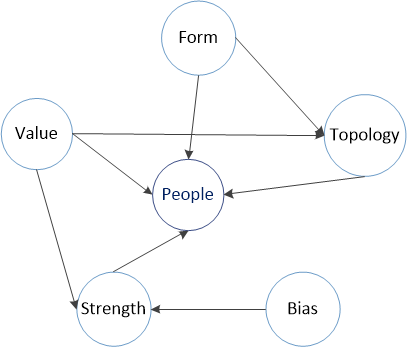
\includegraphics[width=7cm]{./picture/2333.png}
		\caption{The Graphic Model}
		\label{fig:The BG Model}
	\end{figure}
\subsection{Analyse}
	\par In this part, some models are given to what is changing people's mind and how to do that. However, they cannot be quantitatively solved. All models might be made to have a large degree of subjective. But the models we adapt reveal a nearly reality.
	\par The AHP judge different factor in a scientific way, while the AHP model does. The graphic model is a new idea to determine how to change, but it’s more subjective.
	
\par 
\section{CONCLUSIONS}
\subsection{Extends}
\subsubsection*{What if ...}
\begin{itemize}
	\item If the rumors of country-turned-pop singer Taylor Swift’s possible engagement had instead happened in 1860, what percentage of the population would know about
	it and how quickly?
	\begin{itemize}
		\item As a matter of fact, there might be few people (less than the population of a state) will know this. What's worse, the time to get this news might be more than a month.
	\end{itemize}
	\item If an important person was assassinated today, how would that news spread?
	\begin{itemize}
		\item People witnessed the incident might post it to the Facebook, Twitter, Wechat, and so on. In the latest case, people will know it in the second day.
	\end{itemize}
	\item If a fake "valuable" news have been spread, how difficult it is to correct it? 
	\begin{itemize}
		\item It's very hard. A re-spreading speed is slower than the first time. Further, people always has a first impression.
		
	\end{itemize}
\end{itemize}
\par 
 
 
\subsection{Strengths and weaknesses}
Like any model,the ones present above has their strengths and
weaknesses. Some of the major points are presented below:

%============================模型=优点====================================
\subsubsection*{Strengths}
\begin{itemize}
	\item {Applies widely}
	\item \textbf{The models possess practicability and value of popularization}
	\item {From the perspective of as many as possible }
	\item {The models are simple and easy to understand}
	\item {Some of the ideas are very new}
\end{itemize}
\subsubsection*{Weakness}
\begin{itemize}
	\item {The models reveal subjectivity to a certain extent}
	\item {Model in the primary stage}
	\item {Many factors are not considered }
	\item {Some calculating principles have not been explain clearly}
	\item {Few data can be put into testing}
	
\end{itemize}
%======================================================================
\subsection{Summary}

To explore the relationship between information's disseminating speed and its inherent value, make clear the revolution of methodology, purpose, and functionality of society's networks, we design some models based on a consideration of 5 periods: 1870s (Newspapers and Telegraph Age), 1920s (Radios Age), 1970s (Televisions Age), 1990s (Early Internet Age) and 2010s (Mobile Internet Age).
\par We divide our discussion into three parts: mode the dissemination, explore the development of dissemination and discuss the influence of the information network. Specifically, we firstly use the SW Model and BA Model. Then, we analysis the two models and combine them with some notions from Neural Networks into a modified model. After that, we discuss the filter modify the model again. This is the basis for our further work. In the second part, we make a prediction model inspired by the logistic model, the GM(1,n) Model and the BP model. We combine them again, using the Grey Model GM(1,n) to predict a total growth, then putting the data into a BA function based on logistic learning curve. Some data is used as validating the model, and some predictions are generated by the model. In the next part, we analysis the factors that change public interest and opinion, and model how to change it. Three models are applied to this part, a principal component analysis (PCA) model to the first problem, and the analytic hierarchy process (AHP) ,a graphic model to the second problem. Different analysis method reveals different facet of a problem, thus we no longer combine these methods.
\par In the last of this essay, we answer some "What if" problems and analysis the strengthens and weakness of all models. The references and appendices are follow.
\newpage






\begin{thebibliography}{99}
	
%\addcontentsline{toc}{section}{References}
\bibitem{1}David A. Freedman (2009). Statistical Models: Theory and Practice. Cambridge University Press. p. 128
\bibitem{2}Walker, SH; Duncan, DB (1967). "Estimation of the probability of an event as a function of several independent variables". Biometrika 54: 167-178. doi:10.2307/2333860
\bibitem{3} Saaty, Thomas L.; Peniwati, Kirti (2008). Group Decision Making: Drawing out and Reconciling Differences. Pittsburgh, Pennsylvania: RWS Publications. ISBN 978-1-888603-08-8
\bibitem{4}Watts, Duncan J.; Strogatz, Steven H. (June 1998). "Collective dynamics of 'small - world' networks". Nature 393 (6684): 440 - 442. 
\bibitem{5}Onnela, J. -P.; Saramaki, J.; Hyvonen, J.; Szabo, G.; Lazer, D.; Kaski, K.; Kertesz, J.; Barabasi, A. -L. (2007). "Structure and tie strengths in mobile communication networks". Proceedings of the National Academy of Sciences 104 (18): 7332-7336
\bibitem{6}Choromański, K.; Matuszak, M.; MiȩKisz, J. (2013). "Scale-Free Graph with Preferential Attachment and Evolving Internal Vertex Structure". Journal of Statistical Physics 151 (6): 1175.

\bibitem{7}Moonchai S, Rakpuang W. A New Approach to Improve Accuracy of Grey Model GMC in Time Series Prediction[J]. Modelling and Simulation in Engineering, 2015, 2015.
\bibitem{8}Hou S Q. Forecasting of Water Resource of China based on Grey Prediction Model[J]. Advance Journal of Food Science and Technology, 2015, 9(5): 389-392.

\bibitem{9}
Saracoglu, B.O. (2013). "Selecting industrial investment locations in master plans of countries". European J. of Industrial Engineering (Inderscience Enterprises Ltd.) 7 (4): 416-441. doi:10.1504/EJIE.2013.055016
\bibitem{10}He Y, Li X, Deng X. Discrimination of varieties of tea using near infrared spectroscopy by principal component analysis and BP model[J]. Journal of Food Engineering, 2007, 79(4): 1238-1242.
\bibitem{11}http://www.people-press.org/2012/09/27/section-1-watching-reading-and-listening-to-the-news-3/
\bibitem{12}http://www.nature.com/nature/journal/v393/n6684/full/393440a0.html
\bibitem{13}
https://en.wikipedia.org/wiki/Principalcomponentanalysis
\bibitem{14}
https://en.wikipedia.org/wiki/Analytichierarchyprocess 

\bibitem{15}https://en.wikipedia.org/wiki/Scale-free-network
\bibitem{16}https://en.wikipedia.org/wiki/Small-world-network
\bibitem{17}https://en.wikipedia.org/wiki/Logistic-regression
\bibitem{18}https://en.wikipedia.org/wiki/Artificial-neural-network
\bibitem{19}http://baike.baidu.com/link?url=Qm-xihbLpYtYMbmzQZGTX9wSVvMSL4lpL7nto1PFVJ2wiGCKMaDMnQ1WORkeY8aqpaCvBE1m5aMq2zkR8xM0FK
\end{thebibliography}

%====================附录导入程序代码==========================================
\begin{appendices}
   



Here are some programmes we used in our model as follow.\\


\textbf{\textcolor[rgb]{0.98,0.00,0.00}{The core codes of the BP Model:}}
\lstinputlisting[language=Matlab]{./code/matlab1.m}


\textbf{\textcolor[rgb]{0.98,0.00,0.00}{The core codes of Grey Prediction model,GM(1,n):}}
\lstinputlisting[language=Matlab]{./code/huise_gm1n.m}
\end{appendices}
